\documentclass[10pt, conference, compsocconf]{IEEEtran}
\usepackage[bookmarks=true]{hyperref}
\usepackage{epsfig}
\usepackage{amsmath,amssymb,amsfonts,latexsym}
\usepackage{enumerate}
\usepackage{xspace}
\usepackage{epsf,picinpar}
\usepackage{varioref}
\usepackage{colortbl,multirow,hhline}
\usepackage{listings}
\usepackage{amssymb}
\usepackage{colortbl,multirow,hhline}
\usepackage{algorithmic}
\usepackage{algorithm}
\usepackage{caption}
\usepackage[normalem]{ulem}
\usepackage{xcolor}
\usepackage{pifont}
\usepackage{xcolor,colortbl}
\usepackage{url}
\usepackage{balance}
\usepackage{graphicx, subfigure}
\usepackage{longtable}
\usepackage{lscape}
\usepackage{multirow}
\usepackage{listings}
\usepackage{framed}
\usepackage{morefloats}
\usepackage[T1]{fontenc}
\usepackage{array}
\usepackage{pdfpages}
\usepackage{fancybox}
\usepackage{amsmath}
\usepackage{flushend}
\usepackage{booktabs}
\usepackage{enumitem}
\usepackage{makecell}
\usepackage{soul}
\usepackage{multirow}
\usepackage{color}

\DeclareRobustCommand{\hlcyan}[1]{{\sethlcolor{cyan}\hl{#1}}}

\renewcommand{\ttdefault}{cmr}

\newcommand{\limit}[1]{\textcolor{red}{\ding{46}~Page limit:~#1}\\}
\newcommand{\todo}[1]{\textcolor{blue}{\ding{46}~#1}} 
\newcommand{\ie}{\emph{i.e.,}\xspace}
\newcommand{\eg}{\emph{e.g.,}\xspace}
\newcommand{\etc}{etc.\xspace}
\newcommand{\etal}{\emph{et~al.}\xspace} 
    
\begin{document}

\title{
	\todo{Are performance scores good indicators for energy efficiency of web apps}
}

\author{
\IEEEauthorblockN{Miguel Morales Exposito}
\IEEEauthorblockA{2618012\\
m.e.miguel@student.vu.nl}
\and
\IEEEauthorblockN{Tanjina Islam}
\IEEEauthorblockA{2609513\\
tanjina012@gmail.com}
\and
\IEEEauthorblockN{Christian Valladares}
\IEEEauthorblockA{2612946\\
cvalladares4837@gmail.com}
\and
\IEEEauthorblockN{Sanjay Sheombar}
\IEEEauthorblockA{2589918\\
s.sheombar@student.vu.nl}
\and
\IEEEauthorblockN{Kwame Chan-Jong-Chu}
\IEEEauthorblockA{2583387 Number\\
kwamsc91@gmail.com}
}

\maketitle

\begin{abstract}

\noindent \textit{Context}. Developers have access to tools like Lighthouse that help them assess the performance of web apps and to guide the adoption of development best practices. When it comes to energy consumption however, these tools seem to be lacking. 

\noindent \textit{Goal}. This research investigates if there is correlation between the performance scores from Lighthouse and the energy consumption of web apps. By proving correlation, the performance scores could help developers guide their development in less energy consuming web apps.

\noindent \textit{Method}. 21 web apps were measured with the Trepn energy profiler and grouped on the performance treatments: Good, Average and Poor. To assess if the energy consumption is related to the fixed performance treatment, we performed the Kruskall Wallis test. We also performed the Spearman's rank correlation test to identify the correlation between the different performance treatments and energy consumption. Furthermore, we performed Dunn's test to identify the pairwise difference among performance treatments. To quantify these differences, we performed Cliff's Delta between the different pair groups to determine the effect size. 

\noindent \textit{Results}. The Kruskall Wallis test resulted in a significant difference between the performance score cut-offs with a p-value of 3.382e-14. We identified a correlation of -0.324 between performance scores and energy consumption; implying that an increase in performance brings about a decrease in energy consumption. Performing Dunn's test, we discovered that there is a significant difference between Good-Poor and Average-Poor, with an effect size of respectively  $d_{Good-Poor} = -0.444$ and $d_{average-poor} =  -0.386$. However, Dunn's test did not show a significant difference between good and average performing web-apps with a p-value of 0.499, and this is also corroborated by a negligible delta value of -0.099. 

\noindent \textit{Conclusions}. We concluded that poor performant web apps consume more energy than web apps with good or average performance levels. However, the performance score alone would not be sufficient in motivating the software developers to build web apps that consume less energy. Performance scores could guide developers in developing less energy consuming web apps, until the treshold for average is reached. \newline
\end{abstract}

\begin{IEEEkeywords}
Empirical Software Engineering, Green Software, Mobile, Lighthouse, Energy Consumption,
\end{IEEEkeywords}

\section{Introduction}

As mobile users increasingly grow to the largest portion of internet users \cite{Rep:Marketshare}, it is important to keep in mind that these consumers of web based applications have different constraints than their personal computer counterparts. One important constraint is the limited battery life of a mobile device \cite{Rep:Batt}.

It has been shown that poor energy usage of mobile application contributes to user's negative evaluation, and may even lead to abandonment \cite{WEBSITE:2}. Considering the large market share of mobile users, this can affect revenues generated by businesses relying on these applications. This insight can be extended to web applications(web apps) which attempt to produce a native app-like experience in order to fulfill user's growing demand of functionality on web pages, while meeting a developer's requirement of portability across platforms.

Despite of the constraints presented by mobile devices, developers continue to push web technologies to deliver higher functionality while managing performance \cite{Rep:State}. Web apps that have a perceived poor performance affect profits and can lead to user abandonment. The BBC lost an additional 10\% of users for every additional second their site took to load \cite{Web:bbc}. Improving the perceived performance is crucial for increasing conversion. Pinterest rebuilt their pages for the sake of performance, realizing a 40\% reduction in perceived wait times, which increased both search engine traffic and sign-ups by 15\% \cite{Web:pinterest}.

To this end, developers have access to tools that help them assess their web app's performance and to guide the adoption of development best practices. Unlike quality requirements such as performance, 'best practices' and development guidelines provided by higher level measurement tools are lacking when it comes to energy efficiency. According to researchers, Application layer research on energy consumption can empower developers to participate in energy conscious development; but, in the context of their research, they identified a knowledge gap and limited tooling that prevented proper assessment of their application \cite{Rep:EnEf}. Without these resources, the energy mismanagement that could be introduced in the development cycle may be overlooked.

In contrast, there exist many performance bench-marking tools which help to close the knowledge gap and make performance improvements more accessible. Lighthouse is one of many bench-marking tools that attempt to make performance auditing more accessible to developers \cite{Web:Lighthouse}.

As a tool, Lighthouse, makes assessments according to the RAIL performance model, which establishes goals based on human perception \cite{Web:Rail}. Human perception in the RAIL model relates to how an application handles four key actions: the response time to a user's input, the rendering performance for animations, optimal idle-time utilization for the sake of responsiveness, and load impact on a web app. Based on the described model, Fig \ref{fig:Lighthouse} shows the metrics Lighthouse uses to score a web app:

\textit{First Contentful Paint} marks the point, when the browser renders the first bit of content and \textit{First Meaningful Paint} marks the point when the page shows its primary content. These metrics provide feedback for users that the page is actually loading. \textit{Time to interactive} measures how long it takes a page to display "useful" content, and the page responds to user interaction within 50 milliseconds.

These metrics are weighed together and ranked in a log-normal distribution of web apps in order to give a score from 0-100.

\begin{figure}[H]
  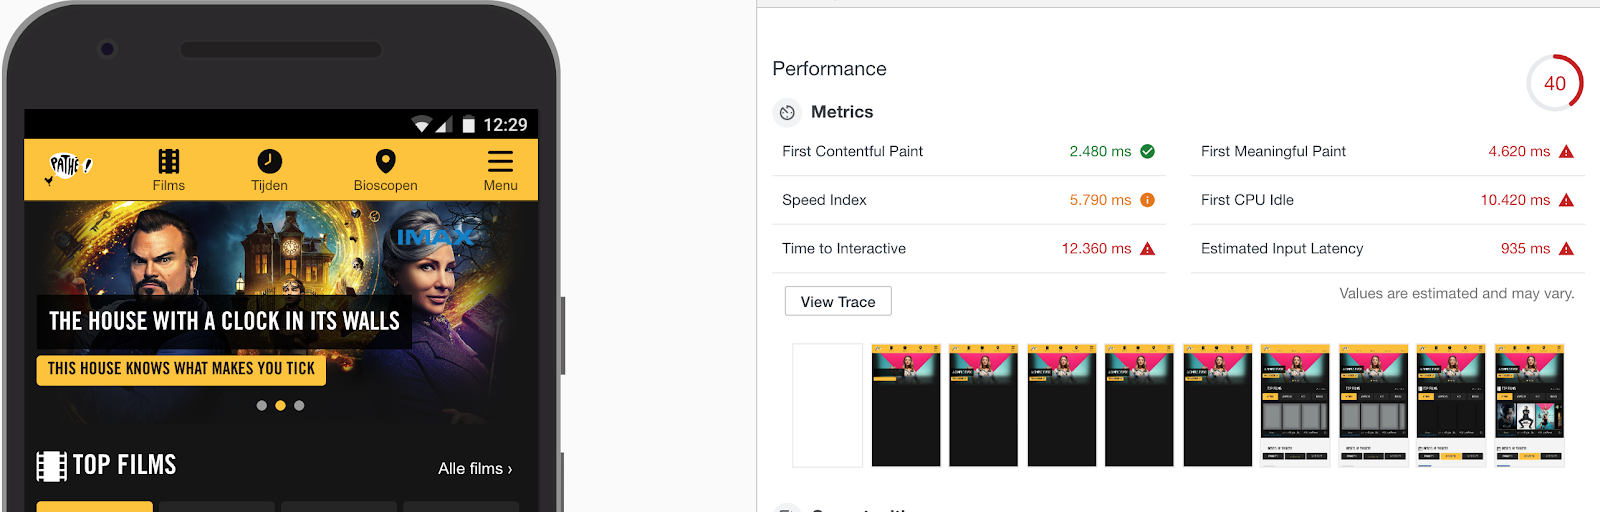
\includegraphics[width=\linewidth]{./Images/lighthousescore.png}
  \caption{Pathe.nl Lighthouse performance audit}
  \label{fig:Lighthouse}
\end{figure}

Energy consumption is overlooked in this assessment. While Web optimizations or any changes to the Web ecosystem are often studied in terms of performance, their effect on energy is not easy to measure. 

The purpose of this research is to analyze if there is a correlation between energy consumption of a web application and its measured performance, and if so, to what extent. A correlation between a high measured performance by these tools and higher energy consumption implies that tools such as these can help guide not only the performance, but also help developers take responsibility for the energy consumption of their web applications.

On the other hand, if there is no correlation, developers can employ this knowledge and use other tools to measure the energy consumption of their application, or even expand Lighthouse to also include an energy consumption meter.
\newline



\section{Experiment Definition}

\subsection{Goal}

The goal of the experiment is identified in Table  \ref{tab:msg1}, using the well-established
GQM goal definition pattern  \cite{Book:Exp}:

\begin{table}[h]                           
    \begin{tabular}{|c|c|}
    \hline

     \textbf{Analyze }   &   Performance Score                \\ \hline
     \textbf{For the purpose of} &   Evaluating correlation             \\ \hline          
     \textbf{With respect to their }    &   Energy Consumption  \\ \hline
     \textbf{From the point of view of}        &   Software Developers         \\ \hline
     \textbf{In the context of}   &   Web Apps           \\ \hline
     \multicolumn{2}{|c|}{\textbf{Result}} \\ \hline
     \multicolumn{2}{|c|}{\makecell{Analyze performance score for the purpose of evaluating how \\ performance correlates with respect to their energy consumption \\ from the point of view of software developers\\  in the context of Web Apps}} \\ \hline

    \end{tabular}
    \caption{Goal definition}
    \label{tab:msg1}                            

\end{table}

\subsection{Questions}

\textbf{[RQ1]}: \textit{To what extent do performance scores correlate to the energy consumption in the context of web apps?}
\newline

To answer this question we will randomly choose 21 web apps from the Alexa list of top visited web apps and load them on the device to measure the energy consumption of each\cite{Web:Alexa}. Then we will compare the energy consumption with the score obtained from Lighthouse and check whether there is any correlation between these two values or not.
\newline

\subsection{Metrics}

To answer the aforementioned questions and thus fulfill the objective of our experiment we will need the following metrics:
\newline

\begin{itemize}
	\item[--] Power consumption: measured in micro-watts.  It is the base metric that we will use to calculate energy consumption of different web apps.
   \item[--] Profiling time: The duration of each run of the experiment, based on the Time to interactive lightouse-metric for each web app in milliseconds.
   	\item[--] Total energy consumption: It is measured in Joule based on power consumption over time to load the web application. This value is calculated using the following formula:
   	 \textit{Energy = Power x Time}   
   	 \newline
\end{itemize}


\subsection{GQM-Tree}

Figure \ref{fig:GQM} displays the visual representation of the GQM tree. This diagram illustrates how our experimental goal, the questions related to this goal and the metrics that are going to address those questions are derived from hierarchical model.
\newline

\begin{figure}[H]
  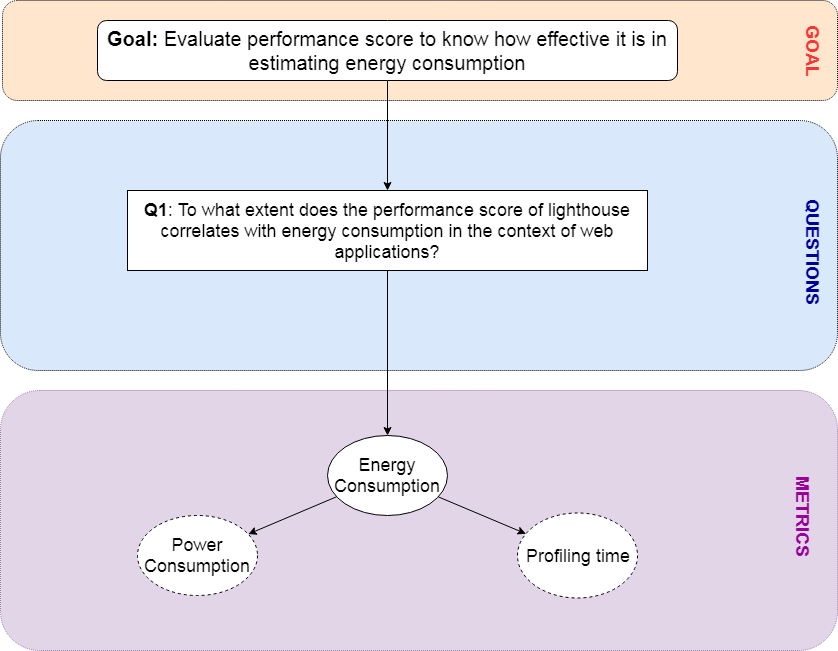
\includegraphics[width=\linewidth]{./Images/GQM.png}
  \caption{GQM tree of the Experiment}
  \label{fig:GQM}
\end{figure}
\newpage



% Please add the following required packages to your document preamble:
% \usepackage{graphicx}
\begin{table*}[]
\resizebox{\textwidth}{!}{%
\begin{tabular}{|l|l|l|l|l|l|l|l|}
\hline
\textbf{App name} & \textbf{URL}               & \textbf{\begin{tabular}[c]{@{}l@{}}Lighthouse \\ Performance \\ Score\end{tabular}} & \textbf{\begin{tabular}[c]{@{}l@{}}Average \\ Energy \\ Consumption\end{tabular}} & \textbf{\begin{tabular}[c]{@{}l@{}}L.o.c.\\ HTML\end{tabular}} & \textbf{\begin{tabular}[c]{@{}l@{}}L.o.c.\\ CSS\end{tabular}} & \textbf{\begin{tabular}[c]{@{}l@{}}L.o.c.\\ JavaScript\end{tabular}} & \textbf{\begin{tabular}[c]{@{}l@{}}Time to \\ interactive\\ (ms)\end{tabular}} \\ \hline
\rowcolor[HTML]{EFEFEF} 
awsamazoncom      & http://www.amazonaws.com   & 0.13 (Poor)                                                                                & 3078.068                                                                          & 11642                                                          & 21519                                                         & 42225                                                                & 26959.452                                                                      \\
apple             & http://www.apple.com       & 0.45 (Average)                                                                                & 175.868                                                                           & 992                                                            & 34967                                                         & 45516                                                                & 6926.777                                                                       \\
\rowcolor[HTML]{EFEFEF} 
ask               & http://www.ask.com         & 0.94 (Good)                                                                                & 39.639                                                                            & 729                                                            & 557                                                           & 11977                                                                & 3364.167                                                                       \\
china*            & http://www.china.com       & 0.08 (Poor)                                                                                & 206.624                                                                           & 2131                                                           & 3617                                                          & 19791                                                                & 14128.010                                                                      \\
\rowcolor[HTML]{EFEFEF} 
cnn               & http://www.cnn.com         & 0.01 (Poor)                                                                                & 2865.623                                                                          & 44803                                                          & 866                                                           & 153037                                                               & 32485.614                                                                      \\
coccoc            & http://www.coccoc.com      & 0.22 (Poor)                                                                                & 537.667                                                                           & 1121                                                           & 16149                                                         & 154126                                                               & 14360.126                                                                      \\
\rowcolor[HTML]{EFEFEF} 
ettoday           & http://www.ettoday.net     & 0.04 (Poor)                                                                                & 477.836                                                                           & 1599                                                           & 15989                                                         & 111295                                                               & 16075.164                                                                      \\
hao123            & http://www.hao123.com      & 0.17 (Poor)                                                                                & 323.192                                                                           & 14582                                                          & 56                                                            & 25905                                                                & 12862.119                                                                      \\
\rowcolor[HTML]{EFEFEF} 
instagram         & http://www.instagram.com   & 0.69 (Average)                                                                                & 141.857                                                                           & 12078                                                          & 0                                                             & 83393                                                                & 5609.320                                                                       \\
microsoft         & http://www.microsoft.com   & 0.86 (Good)                                                                                                                                                               & 55.150                                                                            & 3275                                                           & 94                                                            & 5548                                                                 & 3775.443                                                                       \\
\rowcolor[HTML]{EFEFEF} 
paypal            & http://www.paypal.com      & 0.63 (Average)                                                                                & 91.660                                                                            & 991                                                            & 8995                                                          & 20302                                                                & 5062.576                                                                       \\
popads            & http://www.popads.net      & 0.94 (Good)                                                                                                                                                               & 0.657                                                                             & 434                                                            & 553                                                           & 7253                                                                 & 2756.281                                                                       \\
\rowcolor[HTML]{EFEFEF} 
quora             & http://www.quora.com       & 0.59 (Average)                                                                                & 197.197                                                                           & 4377                                                           & 51492                                                         & 25800                                                                & 7745.406                                                                       \\
theguardian       & http://www.theguardian.com & 0.43 (Poor)                                                                                & 780.819                                                                           & 1337                                                           & 10785                                                         & 48699                                                                & 13140.618                                                                      \\
\rowcolor[HTML]{EFEFEF} 
tianya            & http://www.tianya.cn       & 0.52 (Average)                                                                                & 61.038                                                                            & 347                                                            & 1409                                                          & 7413                                                                 & 5156.529                                                                       \\
twitter           & http://www.twitter.com     & 0.48 (Average)                                                                                                                                                                & 191.287                                                                           & 1616                                                           & 30451                                                         & 54336                                                                & 7372.841                                                                       \\
\rowcolor[HTML]{EFEFEF} 
whatsapp          & http://www.whatsapp.com    & 0.63 (Average)                                                                                & 224.850                                                                           & 20532                                                          & 44333                                                         & 129280                                                               & 7255.729                                                                       \\
xnxx              & http://www.xnxx.com        & 0.8 (Good)                                                                                                                                                                & 124.761                                                                           & 4350                                                           & 10635                                                         & 11023                                                                & 5839.859                                                                       \\
\rowcolor[HTML]{EFEFEF} 
xvideos           & http://www.xvideos.com     & 0.76 (Good)                                                                                                                                                               & 223.455                                                                           & 5381                                                           & 25369                                                         & 23090                                                                & 6610.909                                                                       \\
yandex            & http://www.yandex.ru       & 0.83 (Good)                                                                                                                                                               & 94.201                                                                            & 20125                                                          & 5054                                                          & 62952                                                                & 5070.721                                                                       \\
\rowcolor[HTML]{EFEFEF} 
youtube           & http://www.youtube.com     & 0.75 (Good)                                                                                                                                                               & 170.904                                                                           & 25540                                                          & 12318                                                         & 163102                                                               & 6091.047                                                                       \\ \hline
\end{tabular}%
}

\caption{Web App Characteristics}
    \label{tab:design}
\end{table*}



\section{Experiment Planning}


\subsection{Context Selection}

In this particular section, we cover our context that is the environment under which we are going to perform our experiments. The context has been defined based on four dimensions proposed by Wohlin et al. \cite{Book:Exp}

The first dimension is Online versus Offline experimentation. The context of our experiment is going to be limited to mobile web apps running on the Google Chrome browser on Android device. This is an offline experiment based on the fact that the measurements are done via tools on web apps that have already been developed and published on the web, and we are not part of the development process.

The second dimension is concerned with students or professionals as subjects. Given that our concern is the energy consumption as a function of a web app's performance score, the subjects of the experiment are developers, who ultimately have a direct impact on both the score and an app's energy efficiency.

The third dimension is the nature of the experiment: toy problems vs real problems. We sampled actual web apps from the Alexa list from different performance categories, thus targeting web apps from a real world context. Furthermore, we will be conducting experiments to address a real world problem - how performance score could be an indication of energy consumption for web apps. If proven so, performance audits might help guide software developers towards developing less energy consuming web apps.

 The fourth dimension is whether our experiment is specific versus general. We are specific because we are conducting our experiment using Lighthouse as performance analyzing tool and Chrome browser on Android platform. The web apps used for the experiment are subjects from the top visited web apps with high traffic. Although we are not targeting other supported tools, browsers and platforms, we are using tools made by high regarded developers and have a good representative sample of the population. More specifically, Chrome captures over 60\% market share \cite{WEBSITE:16}. Lighthouse is developed by Google, under active development to improve its audits. Finally, Trepn was developed by Qualcomm which captures 42 percent of processors market share \cite{WEBSITE:17}. \newline


\subsection{Variable Selection}

For our research question, we consider a web app's performance score as the independent variable. We control and change our independent variables via the selection of web apps on the basis of their scores. The measurement scale for this variable is a composite score of different loading time milestones, measured in milliseconds, which are weighted, and these are compared to a benchmark of real web apps. The outcome of this process is a relative performance score placed in a log normal distribution of benchmark scores. 
The scoring range is thus between a score of one and one hundred. We concern ourselves in measuring web apps with the following fixed levels based on lighthouse score ranges \cite{WEBSITE:13}

\begin{itemize}
\item Poor: (0 - 44)
\item Average: (45 - 74)
\item Good: (75 - 100)
\newline
\end{itemize}

We consider the energy consumption as the dependent variable. We measure the consumed energy of a web app while loading it. Energy consumption is a variable calculated as the power consumed by Google Chrome to load one subject multiplied by the time the profiler has been tracking it.
\newline


\subsection{Hypothesis Formulation}
The following hypothesis were formulated to address the main research question.
To assess if the outcome of the energy consumption is related to the fixed performance levels: Poor, Average, Good - we have the following hypothesis: \newline

We test the null hypothesis that the energy consumption mean of web apps in the category low, average and high are the same: 

\[ H_0^1: \mu_{low} = \mu_{average} = \mu_{high} \]
versus the alternative that they are not the same for at least one pair: \[ H_{a}^1: \exists (i,j) | \mu_{i} != \mu_{j} \] for at least one pair (i,j). proving that they are not the same gives an idea of dependency.

\subsection{Subject Selection}
	
	The subject selection is done by a python script \cite{WEBSITE:11} which reads a csv containing the top 1 million web apps from Alexa. The script starts from the first web apps (the most visited measured by Alexa) and goes down the list until it has 100 web apps. We discard domain names where the only difference is their extension. For example if the list contains http://www.google.com and then http://www.google.ru will not be added to the list.
We use Lighthouse batch reporter to run Lighthouse tests on the list of 100 web apps, which generates 100 JSON files with Lighthouse scores \cite{WEBSITE:12}. 
We then place the web apps in categories based on their scores, these categories being poor 0-44, average 45-74, good 75-100. From each of these categories we randomly selected 7 web apps (yielding a total of 21 web apps). \newline
	
\subsection{Experiment Design}


In order to determine if there is any statistically significant
difference between the performance scores, the design will guide the statistical test needed. The statistical test is used to understand whether the energy consumption differed based on the performance score levels.

The process of selecting the right test involves considering the dependent, independent variable and proving the assumptions. 

-Energy consumption of the web app is our dependent variable which is a continuous ratio level of measurement.

-Performance score is our only independent variable with 3 treatments (Good, Average and Poor). \newline

We consider a balanced design of subjects over the different treatments, as shown in Table \ref{tab:design}. Every Treatment level contains 7 unique web apps denoted by $w_i$. Based on this design, we can consider the following tests which rely on the probability distribution of the data.


When the data meets the assumption of the outcome being sampled independently from normal populations, with possibly different population means, and with equal populations variances, we can consider one-way ANOVA. 

When the data does not meet these assumptions, Kruskal Wallis can be considered. \newline

	
\subsection{Instrumentation}

\textbf{Hardware}

For our experiment, we are using Nexus 9 tablet running on Android 5.1.1. The device is equipped with a 2.3 GHZ Dual Core processor (Denver), 2GB of RAM, a Kepler DX1 GPU and a 802.11 a/b/g/n/ac WiFi interface. Furthermore the device has a 6700 mAh Lithium-Polymer battery installed. \newline

\textbf{R and R studio}

R Studio is an IDE for R. It will be used to perform the statistical tests \cite{WEBSITE:14}. \newline

\textbf{Lighthouse}

Lighthouse is used for performance measuring. This tool simulates an Android device and loads a web app on it measuring different audits. It gives a performance score from 0 to 100 based on the specified audits.
 \newpage

\textbf{Trepn}

To measure the energy consumption we use a power and performance profiling application called 'Trepn'. This profiler estimates the energy consumed on the mobile device. To get a better indication of energy consumption of the web app, we selected the delta power consumption value in $\mu W$ which removes the drainage cause by the Android OS and the Trepn profiler itself. From Trepn we will also get the Profiling time in milliseconds. Then, Power consumption and Profiling time will be used to measure the total Energy consumption of each web apps. Web apps are run within the Google Chrome browser (version: 40.0.2214.89) with Javascript V8 3.30.33.15. \newline

\textbf{Android Runner}

For the automation of the experiment, we are using the software tool Android Task runner \cite{WEBSITE:10}. This tool will load each web app on Google Chrome and start the power profiler. After 60 seconds, the browser is closed and Trepn stops profiling. For each web app the test is performed 25 times. The energy consumption is measured for the initial load of the web app, no user interactions will be done on a web app.
\newline


\textbf{Lighthouse Batch Reporter}

This tool is used to perform a Lighthouse analysis on several web apps sequentially. We used to get the performance score of each of our selected subjects \cite{WEBSITE:12}.

\begin{figure*}
  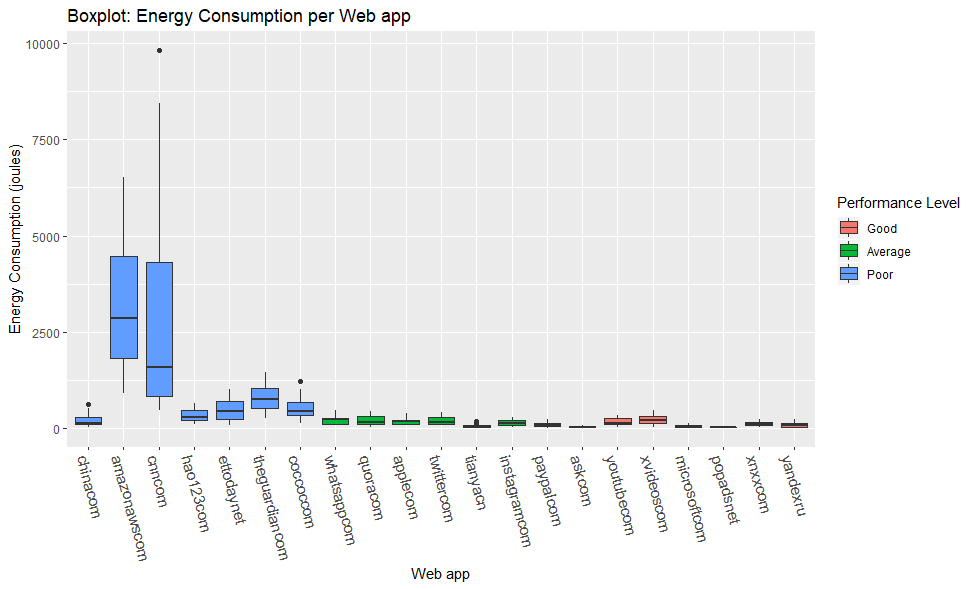
\includegraphics[width=\textwidth]{./NewImages/Fig_3_Boxplot_for_All_Websites.png}
  \caption{Boxplots}
  \label{fig:boxplots-all}
\end{figure*}
\section{Experiment Execution}
Our experiment starts with the setup. Android Runner is executed on a laptop with Ubuntu 18.04.1 LTS, Intel i7-4702MQ and 8GB RAM. With the laptop connected to the Android devices via USB, all the runs will be executed from the laptop.The runs of the experiment are done on the same wifi network with a speed of 100 Mbps. To ensure that the wifi conditions do not alter the experiment output, the mobile device is always placed 5 meters from the router.

We picked the first 100 web apps from the top 1 million Alexa list. We used Lighthouse-batch to get the JSON files with the report of Lighthouse. This returns JSON files which contain the scores of the performance test. We enforce the simulation of 3G connectivity and we also force the simulation of first-time loads (ignoring the cache). This simulation delivers a full report: an aggregated score for each performance category, and also the raw values for each individual load time milestone, in addition to the settings and parameters that were requested for a given test run. The aggregate performance score is the relevant independent variable, thus it is extracted from these reports. 

From these 100 web apps, we randomly select a web app and fill it in a category: Good, Average, Poor, based on its score. This is done until each category reaches 7 web apps. If the randomly selected web app fits a category that already reached its limit of 7, it is discarded. The web apps are ready to use when a total of 21 subjects are selected

From the selected 21 web apps, we run the tests using Android runner which will execute each web app on Google Chrome. \hlcyan{We make the tests with a duration of 60 seconds on intervals of 2 minutes between each run. For the experiment consider the energy consumed up to the first-time-interactive metric given by lighthouse for each web app in order to not punish web apps that load in less than 60 seconds }.  We collect the energy readings using an automated script to execute 21 web apps for 25 trials each. On each run, Android runner will also start the Trepn profile tool and generate a csv file with the power consumed. 
 
Given the design of the experiment, we must take statistical tests for one factor and more than two treatments. The measurements are independent from each other, and energy consumption is a continuous function. We must then analyze  the distribution of these variables in order to check whether a parametric or non-parametric test will hold.  We start with identifying outliers by using a box plot. Furthermore, we intend to use Q-Q Plots with respect to the normal distribution in conjunction with the Shapiro - Wilks test to verify the normality of the dependent variable. We will also verify the normality of the residuals. We will then verify the whether or not an equal variance exists between all sample groups. The parametric checks may not hold initially. In some cases, transforming the data may fit the assumptions better. 

\hlcyan{Upon verifying these assumptions, we will perform either the one-way ANOVA test or Kruskal-Wallis on the collected data. This test will verify whether the means of the different performance score groups stem from unequal population variances. If indeed the population variances differ, we intend to perform Tukey's or Dunn's test to identify which scoring groups differ from each other.  Furthermore, we would like to understand the effect size if indeed an effect exists. This will be done by applying Cohen's d.}

\newpage
\section{Results} 
\subsection{descriptive statistics}
The summary presented in Table \ref{tab:table3} and histogram in Fig \ref{fig:histec} show a better understanding of the energy consumption data of web apps. 

\begin{table}[h!]
  \begin{center}
    \begin{tabular}{l|r} % <-- Alignments: 1st column left, 2nd middle and 3rd right, with vertical lines in between
      \textbf{  } & \textbf{Energy consumption} \\
      \hline
      Min & 3.543\\
      1st Qu. & 71.025\\
      Median & 153.555\\
      Mean & 480.398 \\
      3rd Qu. & 362.120 \\
      Max & 9820.064 \\
      St. deviation & 1080.97\\
    \end{tabular}
        \caption{Summary energy consumption.}
           \label{tab:table3}
  \end{center}
\end{table}


The energy consumption is between 3.543 joules and 9820.064 joules. The central tendency based on the median lies around 153.555 joules. Using the skewness formula \cite{Rep:e1071}, we are able to quantify the skewness of the data. We tested for skewness and achieved a result of 4.77. This value demonstrates a positive skewness as values that deviate from zero implies that the data is not symmetrical. This is further corroborated by the shape of fig \ref{fig:histec}, with the data showing a long tail towards the higher energy consumption values. A standard deviation of 1080.97 joules shows that there is a big spread in the data. 

\begin{figure}[H]
  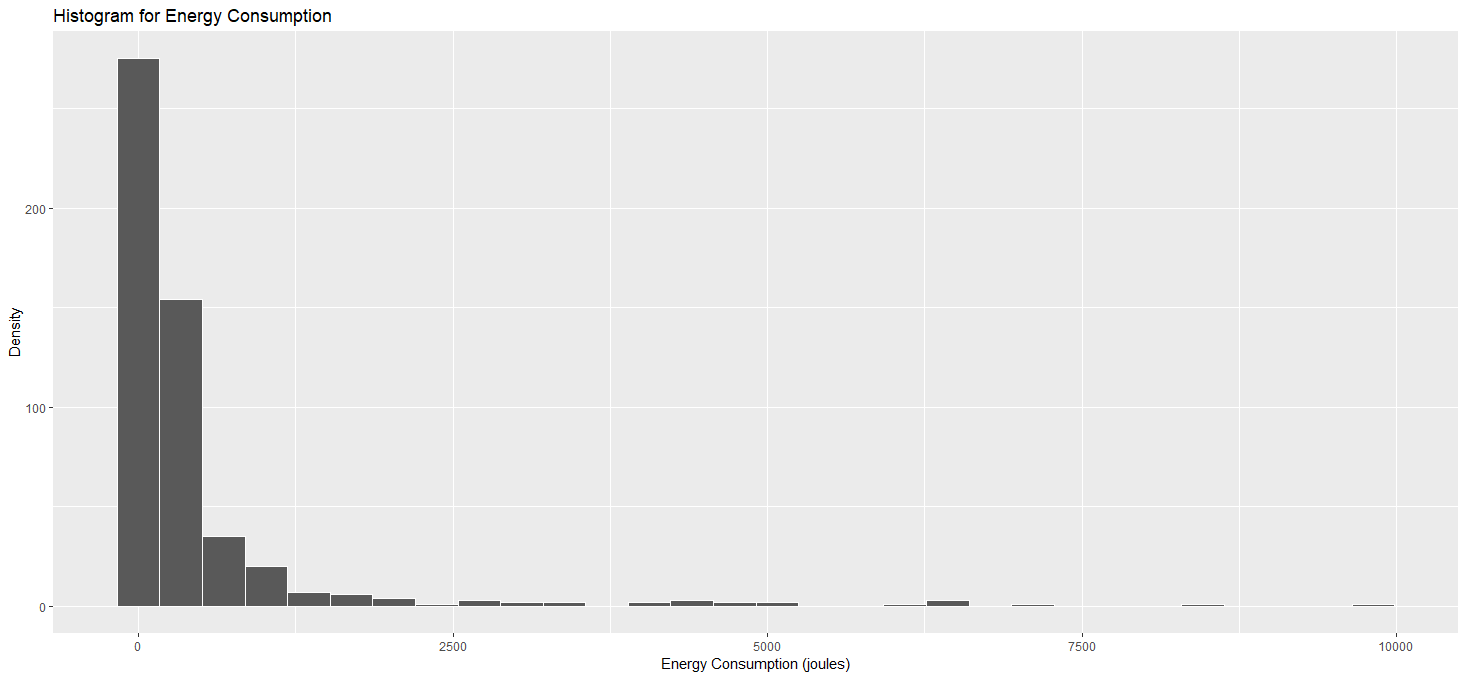
\includegraphics[width=\linewidth]{./NewImages/Fig_4_Histogram_Energy_Consumption.png}
  \caption{Histogram energy consumption}
  \label{fig:histec}
\end{figure}

To get a clearer sense of the observations, we zoomed in on the energy consumption per level in Fig. \ref{fig:boxecv} and Fig. \ref{fig:scatpvsec}. We created energy-consumption box plots diagrams and scatter-plots for the performance levels Good, Average and Poor.

\begin{figure}[H]
  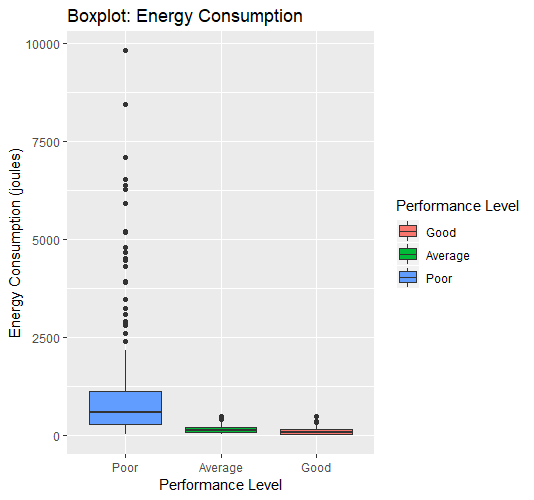
\includegraphics[width=\linewidth]{./NewImages/Fig_5_Box_Plot_Energy_Per_Level.png}
  \caption{Box-plot energy consumption per treatment}
  \label{fig:boxecv}
\end{figure}

\begin{figure}[H]
  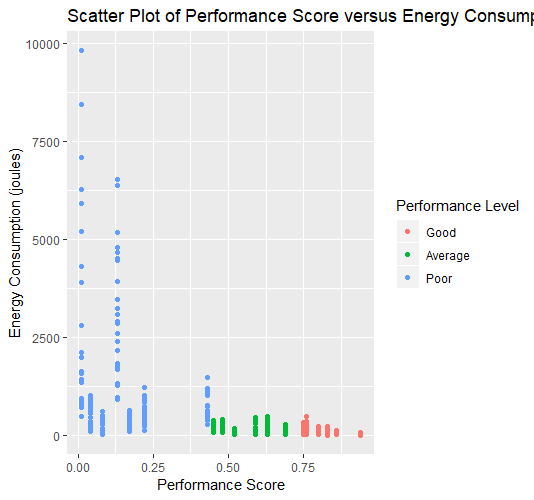
\includegraphics[width=\linewidth]{./NewImages/Fig_6_Scatterplot_Perf_score_Energy.png}
  \caption{Scatter-plot performance vs energy consumption}
  \label{fig:scatpvsec}
\end{figure}

From the diagrams, we could see that the energy consumption measurements for Good and Average are pretty similar; both of these groups are centered around the same energy consumption value, and their outliers are quite similar. Comparing both the good and average performance values to the Poor performance level, we see a bigger difference. The median energy consumption from poor performing web apps is higher when compared to good and average performance web apps. \newline

The histogram for energy consumption in Fig. \ref{fig:histec} indicates that the energy consumption data is not normal. To justify our assumption we performed a Q-Q plot against a random sample of the normal distribution in Fig. \ref{fig:qqec}.

\begin{figure}[H]
  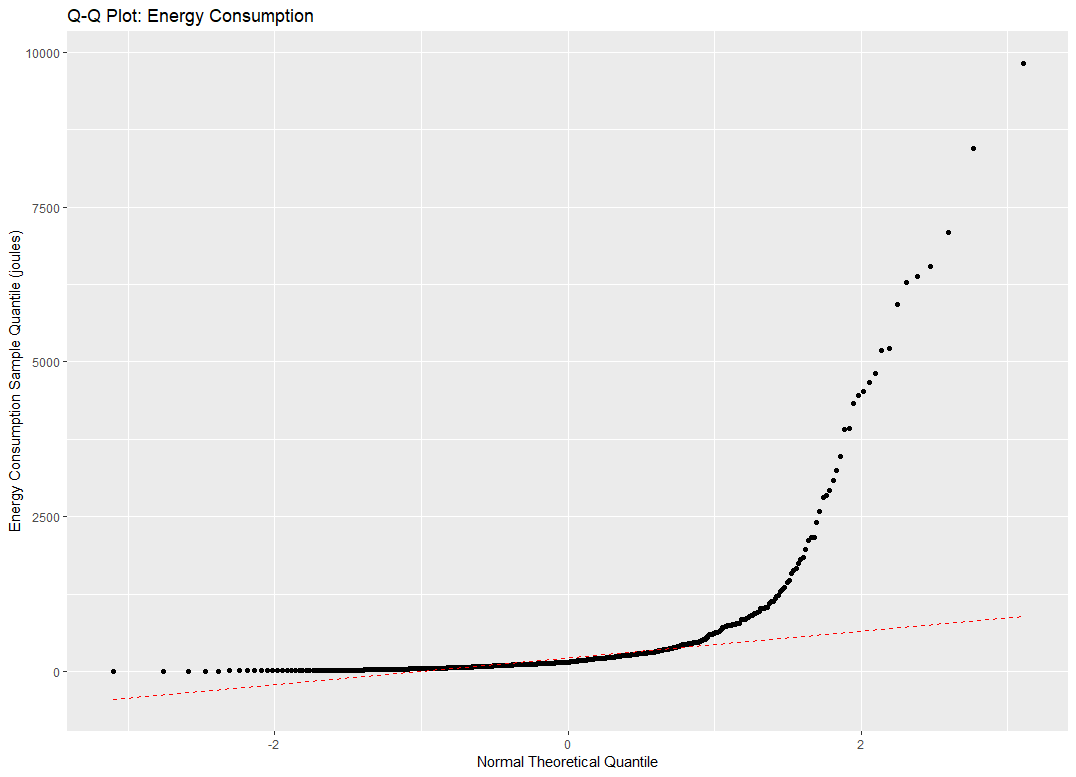
\includegraphics[width=\linewidth]{./NewImages/Fig_7_QQPLOT_RAW.png}
  \caption{Q-Q-plot energy consumption}
  \label{fig:qqec}
\end{figure}

The assumption of non normality for the energy consumption data could be caused by the rather small sample size of 21 web apps, or extreme values caused by the distortion of the data. We would prefer to use parametric statistics based on the higher statistical power of these tests. We performed various data transformations on the energy consumption data, including the squared (Fig. \ref{fig:histqq-sqr}), reciprocal (Fig. \ref{fig:histqq-rec}), and the log transformation of the collected data (Fig. \ref{fig:histqq-log}). The most promising transformation is the log operation on the energy consumption sample:

\begin{figure}[H]
  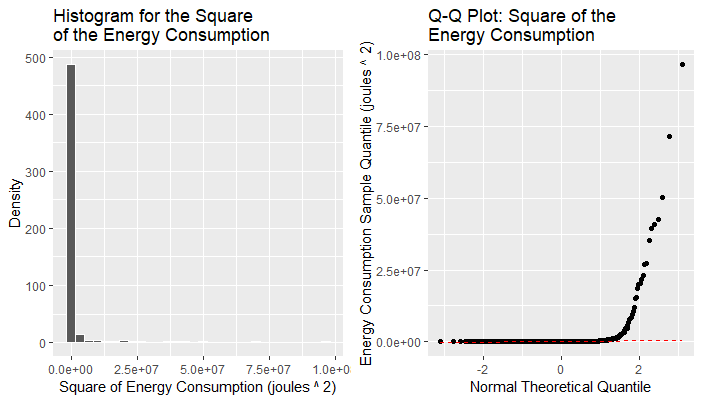
\includegraphics[width=\linewidth]{./NewImages/Fig_8_Squared_Transform.png}
  \caption{Squared transformation for energy consumption}
  \label{fig:histqq-sqr}
\end{figure}

The square transformation of the energy consumption exacerbated the skewness of the data to a skewness value of 6.669, and this is clearly seen from both the histogram and the Q-Q plot.  The Histogram does not show the characteristic bell-shape of normal data and the Q-Q plot demonstrates a more pronounced curvature.


\begin{figure}[H]
  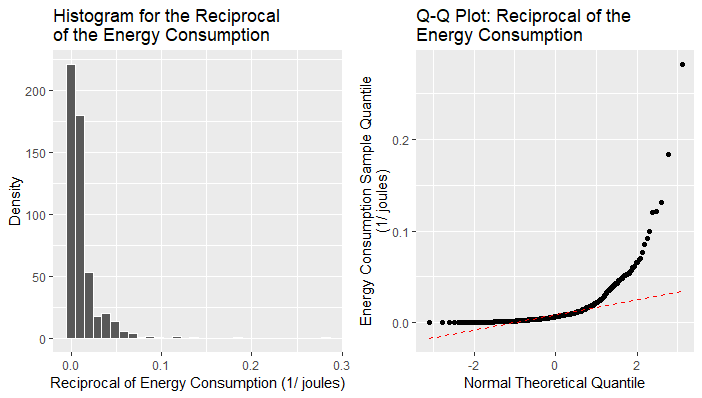
\includegraphics[width=\linewidth]{./NewImages/Fig_9_Reciprocal_Transform.png}
  \caption{Reciprocal transformation for energy consumption}
  \label{fig:histqq-rec}
\end{figure}

The reciprocal transformation was able to better approximate our data to a normal distribution. Skewness decreased to a value of 1.646. However, the curvature of the Q-Q plot is still quite pronounced.

\begin{figure}[H]
  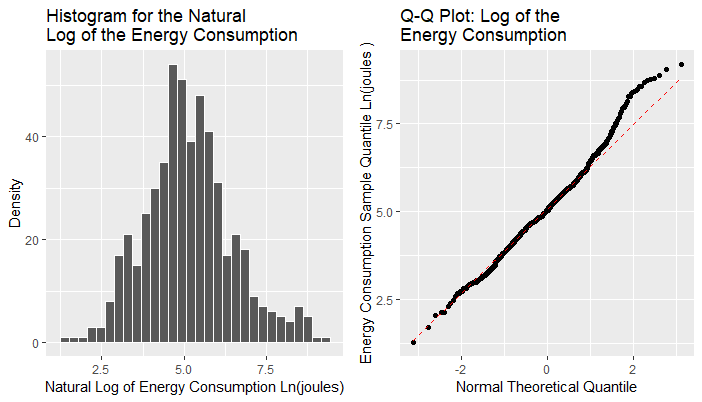
\includegraphics[width=\linewidth]{./NewImages/Fig_10_Log_Transform.png}
  \caption{Log transformation for energy consumption}
  \label{fig:histqq-log}
\end{figure}

We check the histogram of the log of the data, and we see that the skewness is dramatically improved. However the data is still positively skewed with an estimated value of 0.421, and the Quantile-Quantile plot shows a slight curvature. Furthermore, we performed the Shapiro - Wilks test, and received a p-value of 1.111e-4, thus there exists evidence to deny the null hypothesis that the transformed data lies within the normal distribution.


\subsection{Hypothesis testing}
As the assumption that the data comes from a normal distribution was not met, we performed the Kruskal Wallis non-parametric test based on our experiment design. 
The Kruskal Wallis rank based non-parametric test is used to determine if there are statistically significant differences between the energy consumptions at the different treatment levels: Good, Average, Poor. Employing the grouping technique from Lighthouse ensures a representative design, given that the performance scores themselves are defined in relation to the scores of other web apps.

In order to perform the test we made a numeric vector for our treatment levels by using a value of 3 for high performing web apps whereas a value of 1 for poor performance level. We got a p-value of 3.382e-14. Therefore, we can reject the null hypothesis that the means of energy consumption for each performance levels are equal.

Then we checked the correlation between the performance score of a web app and its energy consumption by using the spearman non-parametric correlation test. We obtained a negative correlation value of -0.324 for energy consumption with respect to performance, which infers that the energy consumption increases as the level of performance drops. 

After that we performed a post-hoc pairwise comparison using Dunn tests due to the non-parametric nature of the data. Given that multiple pairwise comparisons are performed, the p-value must be corrected to avoid the higher probability of getting statistically significant results by chance.  We used the Bonferroni correction technique for the pairwise comparison test. We got a p-value of 3.888e-13 for comparison between good and poor and a p-value of 5.119e-09 between average and poor performance levels. This results show that  there is significant difference between good versus poor and average versus poor performance levels. On the other hand, we got a p-value of 0.499 between good and average levels, therefore we cannot assume a significant difference for these two treatments.

Next we applied Cliff's delta to investigate the effect size. Effect size will help us to know the quantified measure of the difference between two groups as it emphasizes more on the size of the difference rather than mixing it up with sample size. By looking at the delta estimate of -0.099  we found that the effect size is negligible when comparing good and average levels. For the comparison between good-poor and average-poor we get delta estimates of -0.444 and -0.386 respectively. These results show that the effect size for those treatment levels is medium.

\begin{figure}[H]
  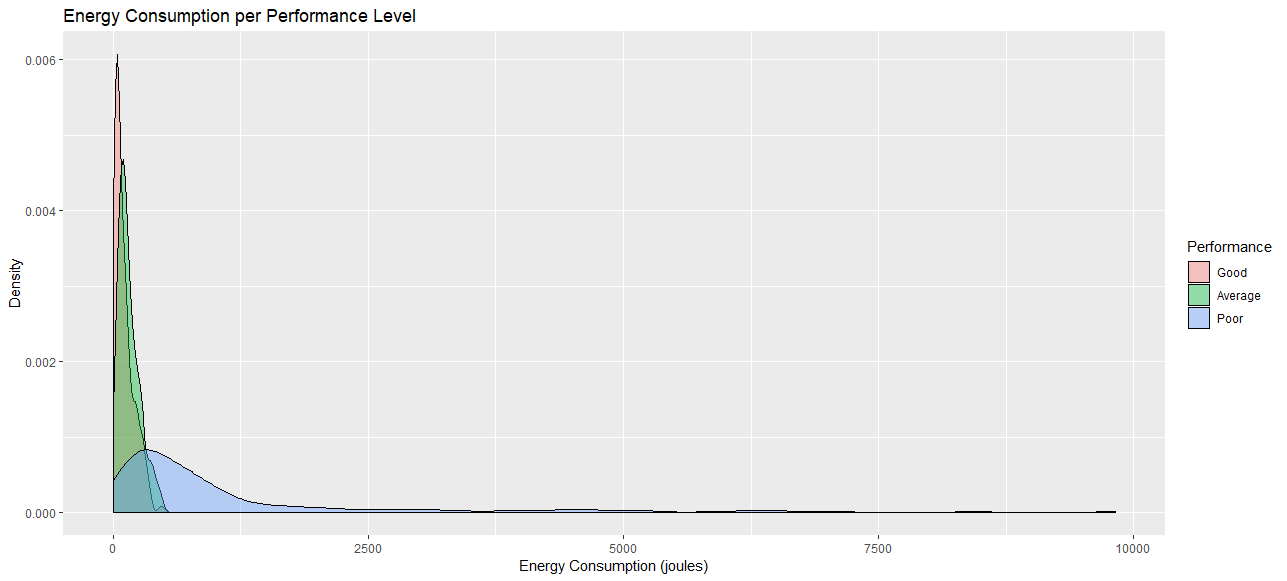
\includegraphics[width=\linewidth]{./NewImages/Fig_11_Density_Curve_Energy_Consumption.png}
  \caption{Density curve for energy consumption}
  \label{fig:density-levels}
\end{figure}

In order to support the results given by Cliff's delta test we depicted in Fig. \ref{fig:density-levels} a density graph with different levels. In this graph we can see how the density of good and average score are very similar and show a high frequency on low energy consumption values. Contrarily, we see smaller frequencies for low energy consumption for the web apps with poor performance score.





\section{Discussion}
From the results of the statistical tests performed in the previous section we can elaborate on our research question. 
The outcome of the Kruskal Wallis test shows that we can reject our null hypothesis. Therefore, we can say that there is a difference in the means of energy consumption of the different performance levels. \newline

Given that Kruskal Wallis is an omnibus statistical test, the nature of these differences is best explained with the Dunn test. With the results from the Dunn test we can see that there is no significant differences of energy consumption between the good and average performance levels of web apps. However, the test shows that the difference in energy consumption of web apps with poor performance levels is quite relevant.
\newline

Finally we try to see the degree of overlap between two distributions of performance levels. With Cliff's Delta test we know that the effect size of a poor performance level against good and average levels is moderate as described by the Cliff's delta guidelines. However, comparing good and average performance levels yields negligible effect sizes. 
\newline

\hlcyan{With the help of data analysis and the obtained results from our experiment we can answer our \textit{research question: To what extent does the performance score of lighthouse correlate with energy consumption in the context of web applications?}}
\newline

\hlcyan{We can conclude that performance score of lighthouse can be used as an indication of how much energy a certain web app consumes. More precisely, we can say that when a web app has a performance score between 0 and 44, the energy consumption is going to be higher than a web app with more than 44 as performance score. }
\newline

\hlcyan{This information can be useful for the web developers who are interested in reducing the energy consumption from their web applications. While developing web apps they can take into account the performance score from lighthouse's performance audit as a guide to estimate how much energy is going to be consumed by that particular web app. And based on this score, they can adopt changes or optimize the codes so that their web app consumes less energy.}



\section{Threats To Validity}\label{sec:threats}
The validity of the experiment has been analyzed based on the four types of classification as defined by Cook and Campbell \cite{Book:Quasi-exp}.The four different types of threats to the validity of our experiment are described in the following sections:

\subsection{Internal Validity}

\textbf{History}

The way we performed the experiments to collect the energy consumption data was incremental. The first three data collection iterations collected energy consumption data on increments of 5 tests per day with two minutes between test. The last iteration was performed 4 days later with a repetition of 10 runs with two minutes between runs. This way we obtained the energy consumption of each web app 25 times. Furthermore, we performed the subject selection based on performance scores a few days before the energy consumption data was collected. Given the time gap between the subject selection and the data collection process, history may be  an internal threat to validity because a web app's performance score could have changed all throughout the data collection process.  
This is also true for the Performance score for a web app.  Given the time constraints, the motivation behind performing a more iterative data collection was to ensure that a balanced data set was produced; we opted for smaller increments so that every web app ended up with an equal number of runs per web app while reducing the risk of not collecting enough data on time. Furthermore, we tried to collect the energy consumption data on iterations as close to each other as possible to mitigate this threat.   \newline


\textbf{Maturation}

Maturation might play a role if a trial is repeated multiple times over same object.  In order to reduce the effect of it, we made sure that Android runner takes intervals of 2 minutes with a duration of 60 seconds between each test execution. After each execution, it also clears up the cache from the web browser. Thereby, even though the trials are applied in different time-frames we made sure that there was not any cached data to influence the second run. \newline

\textbf{Reliability of measures}

There are several factor that can affect the reliability of the measures i.e. brightness of the devices, distance to the router and interference with other processes consuming energy. To mitigate this, we always set the brightness of the screen to the minimum and always set the device at the same distance from the router. To ensure that the energy measured is only consumed by the web app under test, we used the delta values for power consumption of Trepn which does not consider the energy consumed by the profiler and the OS. Furthermore, we have only considered the energy consumed by each web app until it is interactive. Using the first-time-interactive we mitigate the risk of punishing web apps that load faster than the profiling time used in Android runner.




\subsection{External Validity}

\textbf{Interaction of selection and treatment}

Since convenience sampling has been chosen as the sampling technique, there is a high chance of introducing biases and therefore it will make the outcome difficult to be generalized. This threat deals with the situation when the population of subjects is not representative of the one for which we would like to generalize our results. The population of the subjects (web apps) was chosen from the Alexa top 1 million web apps in terms of high traffic. We randomly selected 21 out of the 100 popular most visited web apps as our representative sample. We sampled the top 100 subset due to their high traffic--thus we select web apps of interest to a general population.  Furthermore, the randomization of the selection process allows us to not introduce biases based on the type of web apps selected.  
Although the specific selection of samples affects the external validity and thus the results obtained from it may not be generalized but however, specific sampling helps to represent the scope of our defined experiment. Which in turn, results in performing the analysis of outcomes much more easier and thus increase the conclusion validity. \newline


\textbf{Interaction of setting and treatment}

This threat deals with the situation when the experiments are performed in such a testing environment which is not realistic. For our experiment we used a relatively new device connected via wifi which representative of the way most users browse the internet. Google Chrome was the mobile browser of choice which captures 60\% of market share and Lighthouse which is supported by Google. By using these tools and materials we made sure to generate a realistic experimental setting environment that is representative of a real world problem.


\subsection{Construct Validity}

\textbf{Definition of constructs}

In order to mitigate inadequate pre-operational explanation of constructs, we defined our constructs quite early before even performing the experiments using the standard GQM method. The goal of our experiment as well as the questions related to this goal and the metrics that are relevant to address those questions have been derived from this well-established GQM- tree. Using the GQM approach, we also formulated the hypotheses to address the main research question and identified the independent and dependant variables for our experiment. \newline

\textbf{Mono-operation bias}

Our experiment is based on one factor, performance score which is the independent variable of our experiment design. Since we have only one independent variable, therefore the experiment might face mono-operation bias. But, we performed our experiments using 25 trials on single factor with 3 treatments which will help to mitigate the mono-operation bias from our measurements.



\subsection{Conclusion Validity}

\textbf{Low statistical power}

In order to deal with this threat and reduce the impact size of it, we made sure to have enough data to perform the data analysis. We used a fixed number of treatments i.e. 3 for our experiments with 7 subjects each. So in total 21 web apps and we executed the test 25 times per web app. Therefore, we have relatively large sample size with 525 trials in total of the web apps for all three treatment levels. This is done to make sure that we have sufficient data to perform statistical analysis on that.  However, for future research, it may be helpful to increase the number of web apps per category to verify if statistically significant differences may be identified between good and average performing web apps. \newline

\textbf{Violated assumptions of statistical tests}

To mitigate this threat to validity, we checked the distribution of data before performing the statistical analysis on that. This is done to make sure that we will select appropriate tests basing on the data distribution type. So that, based on the distribution of data, we can adjust our tests accordingly. While formulating our experiment plan, we decided to use the ANOVA test assuming the energy consumption is normally distributed. In our case this was not true hence we adjusted our tests and migrated to Kruskal-Wallis test. \newline

\textbf{Fishing and error rate}

Since convenience sampling has been chosen as the sampling technique, there is a high chance of introducing biases and therefore it could influence the outcomes of our experiment. However, the specific selection of samples helps to define the scope of the experiments and thus will help to answer our research questions. But apart from that, with regards to mitigate this threat to validity we applied Bonferroni's p-value correction technique to obtain statistical correctness so that we can adapt the significance difference that we found while performing different statistical tests. 

\section{Conclusions}\label{sec:conclusions}

In this article we study the relation between performance score given by lighthouse and the energy consumption of a web app. We designed an experiment with performance score as a factor and three different treatment levels according to the performance category. After conducting the experiments, our results show that web apps with a poor performance score consumes more energy than web apps with good or average performance. Also, the energy consumption for web apps with good performance is significantly smaller than those with average performance; nonetheless, this difference is not as large when compared toe the difference with poor performance web apps. \newline 

Looking into the obtained results, we can see how lighthouse can be used in a promising way to measure and assess the consumed energy. Lighthouse can not only assess, but also provides guidance on how to improve critical performance aspects. Considering this, we recommend the developers to use this tool to set development milestones to improve the web app's performance. In doing so,  developers will increase the likelihood of lowering the energy consumption of their web app, as showed by this research.
\newline

Apart from that, this experiment could be extended performing an analysis on the score of each of the audits used to give a performance score. This way it would be possible to know which audit affects more to the energy consumption and developers could focus on its improvement to reduce energy consumption. \newline

Another possible extension to the study could be done by using different bench-marking tools. In this way, it would be possible to know which tool gives a more precise score to estimate energy consumption.



\bibliographystyle{IEEEtran}
\bibliography{refs.bib}

\end{document}
